\section{Methods}

%%%%%%%%%%%%%%%%%%%%%%%%%%%%%%%%%%%%%%%%%
% Morphology and physiology of neuron classes
\subsection{Morphology and physiology of neuron classes}

%% Intro
Seven excitatory pyramidal cell and two interneuron cell models were employed in the network. Their morphology and physiological responses are summarized in \fref{fig_pops}.

%% Detailed PT and IT cells
In previous work we developed layer 5B PT corticospinal cell and L5 IT corticostriatal cell models that reproduce in vitro electrophysiological responses to somatic current injections, including sub- and super-threshold voltage trajectories and f-I curves \cite{Neym17,Sute13}. To achieve this we optimized the parameters of the Hodgkin-Huxley neuron model ionic channels -- Na, Kdr, Ka, Kd, HCN, CaL, CaN, KCa -- within a range of values constrained by literature. The corticospinal and corticostriatal cell model morphologies had 706 and 325 compartments, respectively, digitally reconstructed from 3D microscopy images. We further improved the PT model by 1) increasing the concentration of Ca2+ channels ("hot zones") between the nexus and apical tuft, following parameters published in \cite{HayS11}; 2) lowering dendritic Na+ channel density in order to increase the threshold required to elicit dendritic spikes, which then required adapting the axon sodium conductance and axial resistance to maintain a similar f-I curve; 3) replacing the HCN channel model and distribution with a more recent implementation by Migliore \cite{Migl12}. The new HCN channel reproduced a wider range of experimental observations than our previous implementation \cite{Kole06}, including the change from excitatory to inhibitory effect in response to synaptic inputs of increasing strength \cite{Geor09}. This was achieved by including a shunting current proportional to \ih\. We tuned the HCN parameters ($lk$ and $v_{rev_lk}$) -- originally developed for a CA3 pyramidal neuron \cite{Migl12} -- and passive parameters to reproduce these experimental findings using the corticospinal cell, while keeping its somatic f-I curve consistent with recordings \cite{Sute13}. 

\note{Tuning corticospinal cell response to ih [next paper?] -- figs 3,4,7 Sheets + fig 1 George/Migliore}


%% Other excitatory cell models
The network model includes five other excitatory cell classes: layer 2/3, layer 4, layer 5B and layer 6 IT neurons and layer 6 CT neurons. Since our focus was on the role of L5 neurons, other cell classes were implemented using simpler models as a trade-off to enable running a larger number of exploratory network simulations. Previously we had optimized 6-compartment neuron models to reproduce somatic current clamp recordings from two IT cells in layers 5A and 5B. The layer 5A cell had a lower f-I slope (X) and higher rheobase (X) than that in layer 5B (X and X). Based on our own and published data, we found two broad IT categories based on projection and intrinsic properties: corticocortical IT cells found in upper layers 2/3 and 4 which exhibited a lower f-I slope (avg X) and higher rheobase (avg X) than IT corticostriatal cells in deeper layers 5A, 5B and 6 (avg X and X) \cite{Yama15,Sute13,Oswa13}. CT neurons' f-I rheobase and slope (X and X) was closer to that of corticocortical neurons \cite{Oswa13}. We therefore employed the layer 5A IT model for layers 2/3 and 4 IT neurons and layer 6 CT neurons, and the layer 5B IT model for layers 5A, 5B and 6 IT neurons. We further adapted cell models by modifying their apical dendrite length to match the average cortical depth of the layer, thus introducing small variations in the firing responses of neurons across layers.

\note{
ADD values of model cells f-I slope and rheobase

- Yamawaki 2015: 
-- f-I slope (Hz/nA): L23=63, L4=80, L5A=103
-- Ithresh (pA): L2/3=267, L4=295, L5A=163

- Suter, 2013 (temp 34ºC):
-- CSTR rheobase: 182 (SPI: 341); 
-- f-I slope (Hz, nA): CSTR= 61, SPI= 98

- Oswa 2013 (temp 26ºC):
-- fI slope (HZ/nA): CSTR=88, SPI=82, CTh=69, CC (upper layers?)=82
-- max feq (Hz): CSTR 29, SPI=34, CTh=26, CC=30
-- I50\%maxfreq (pA): CSTR=214 (15hz), SPI=273 (17hz), CT=486 (13Hz) , CC=332 (15hz)
-- at 34ºC all higher -- CSPI higher rates than rest

*** use 1 for upper layers, and other for lower
- IT2, IT4, CT6 use simple BS1578 with adapted L (higher rheobase/Ithresh, smaller fI slope; Yamwaki 2015, Oswa 2013)
- IT5A, IT5B, IT6 use simple/detailed BS1579 (lower rheo, higher fi slope; Yamawaki 2015, Suter 2013, Oswa 2013)
- (not using detailed BS1578) - differentiate upper (1578) vs lower (1579) ITs; and lower IT (1579) vs CT (1578)
*** use detailed IT only for L5A ??
- strong connections to IT L5A not 5B
- use detailed BS1579 for IT L5A; reduced BS1579 for IT L5B

- several diffs: eg. CT input resistance lower than IT + PT; sag higher than IT + PT; more adaptation than IT+PT ...

- in model, higher rheobase + lower firing rates: evidence in OSwa 2013 (I50\% significantly higher ~480pA vs ~250pA; no rheobase values)
}

%% Inhibitory cell models
We implemented models for two major classes of GABAergic interneurons \cite{Harr15}: parvalbumin-expressing fast-spiking (PV) and somatostatin-expressing low-threshold spiking neurons (SOM). We employed existing simplified 3-compartment (soma, axon, dendrite) models \cite{Kons14} and increased their dendritic length to better match the average f-I slope and rheobase experimental values of cortical basket (PV) and Martinotti (SOM) cells (Neuroelectro online database \cite{Trip15}). 
\note{mention properties of each interneuron?}

\note{
- Missing other major group of GABAergic interneurons that express the serotonin receptor,5HT3aR  \cite{Rudy11,Harr15}
- Include VIP and neurogliaform
- Less well characterized \cite{Naka16}
- Overall accounts for ~30\%: 50\% in L2/3 but only ~10-15\% of deeper layers \cite{Rudy11}; 10-25\% of L5 \cite{Katz11,Naka16}
- VIP distribution: L1: 9.8\%, L2/3: 39.3\%, L4: 34.4\%, L5A: 9.8\%, L5B: 6.6\%, L6: 0\% \cite{WallD16}
}

%% Figure: IT,PT tuning; f-I curves all cells
\begin{figure}[!h]  %% bht
\centering
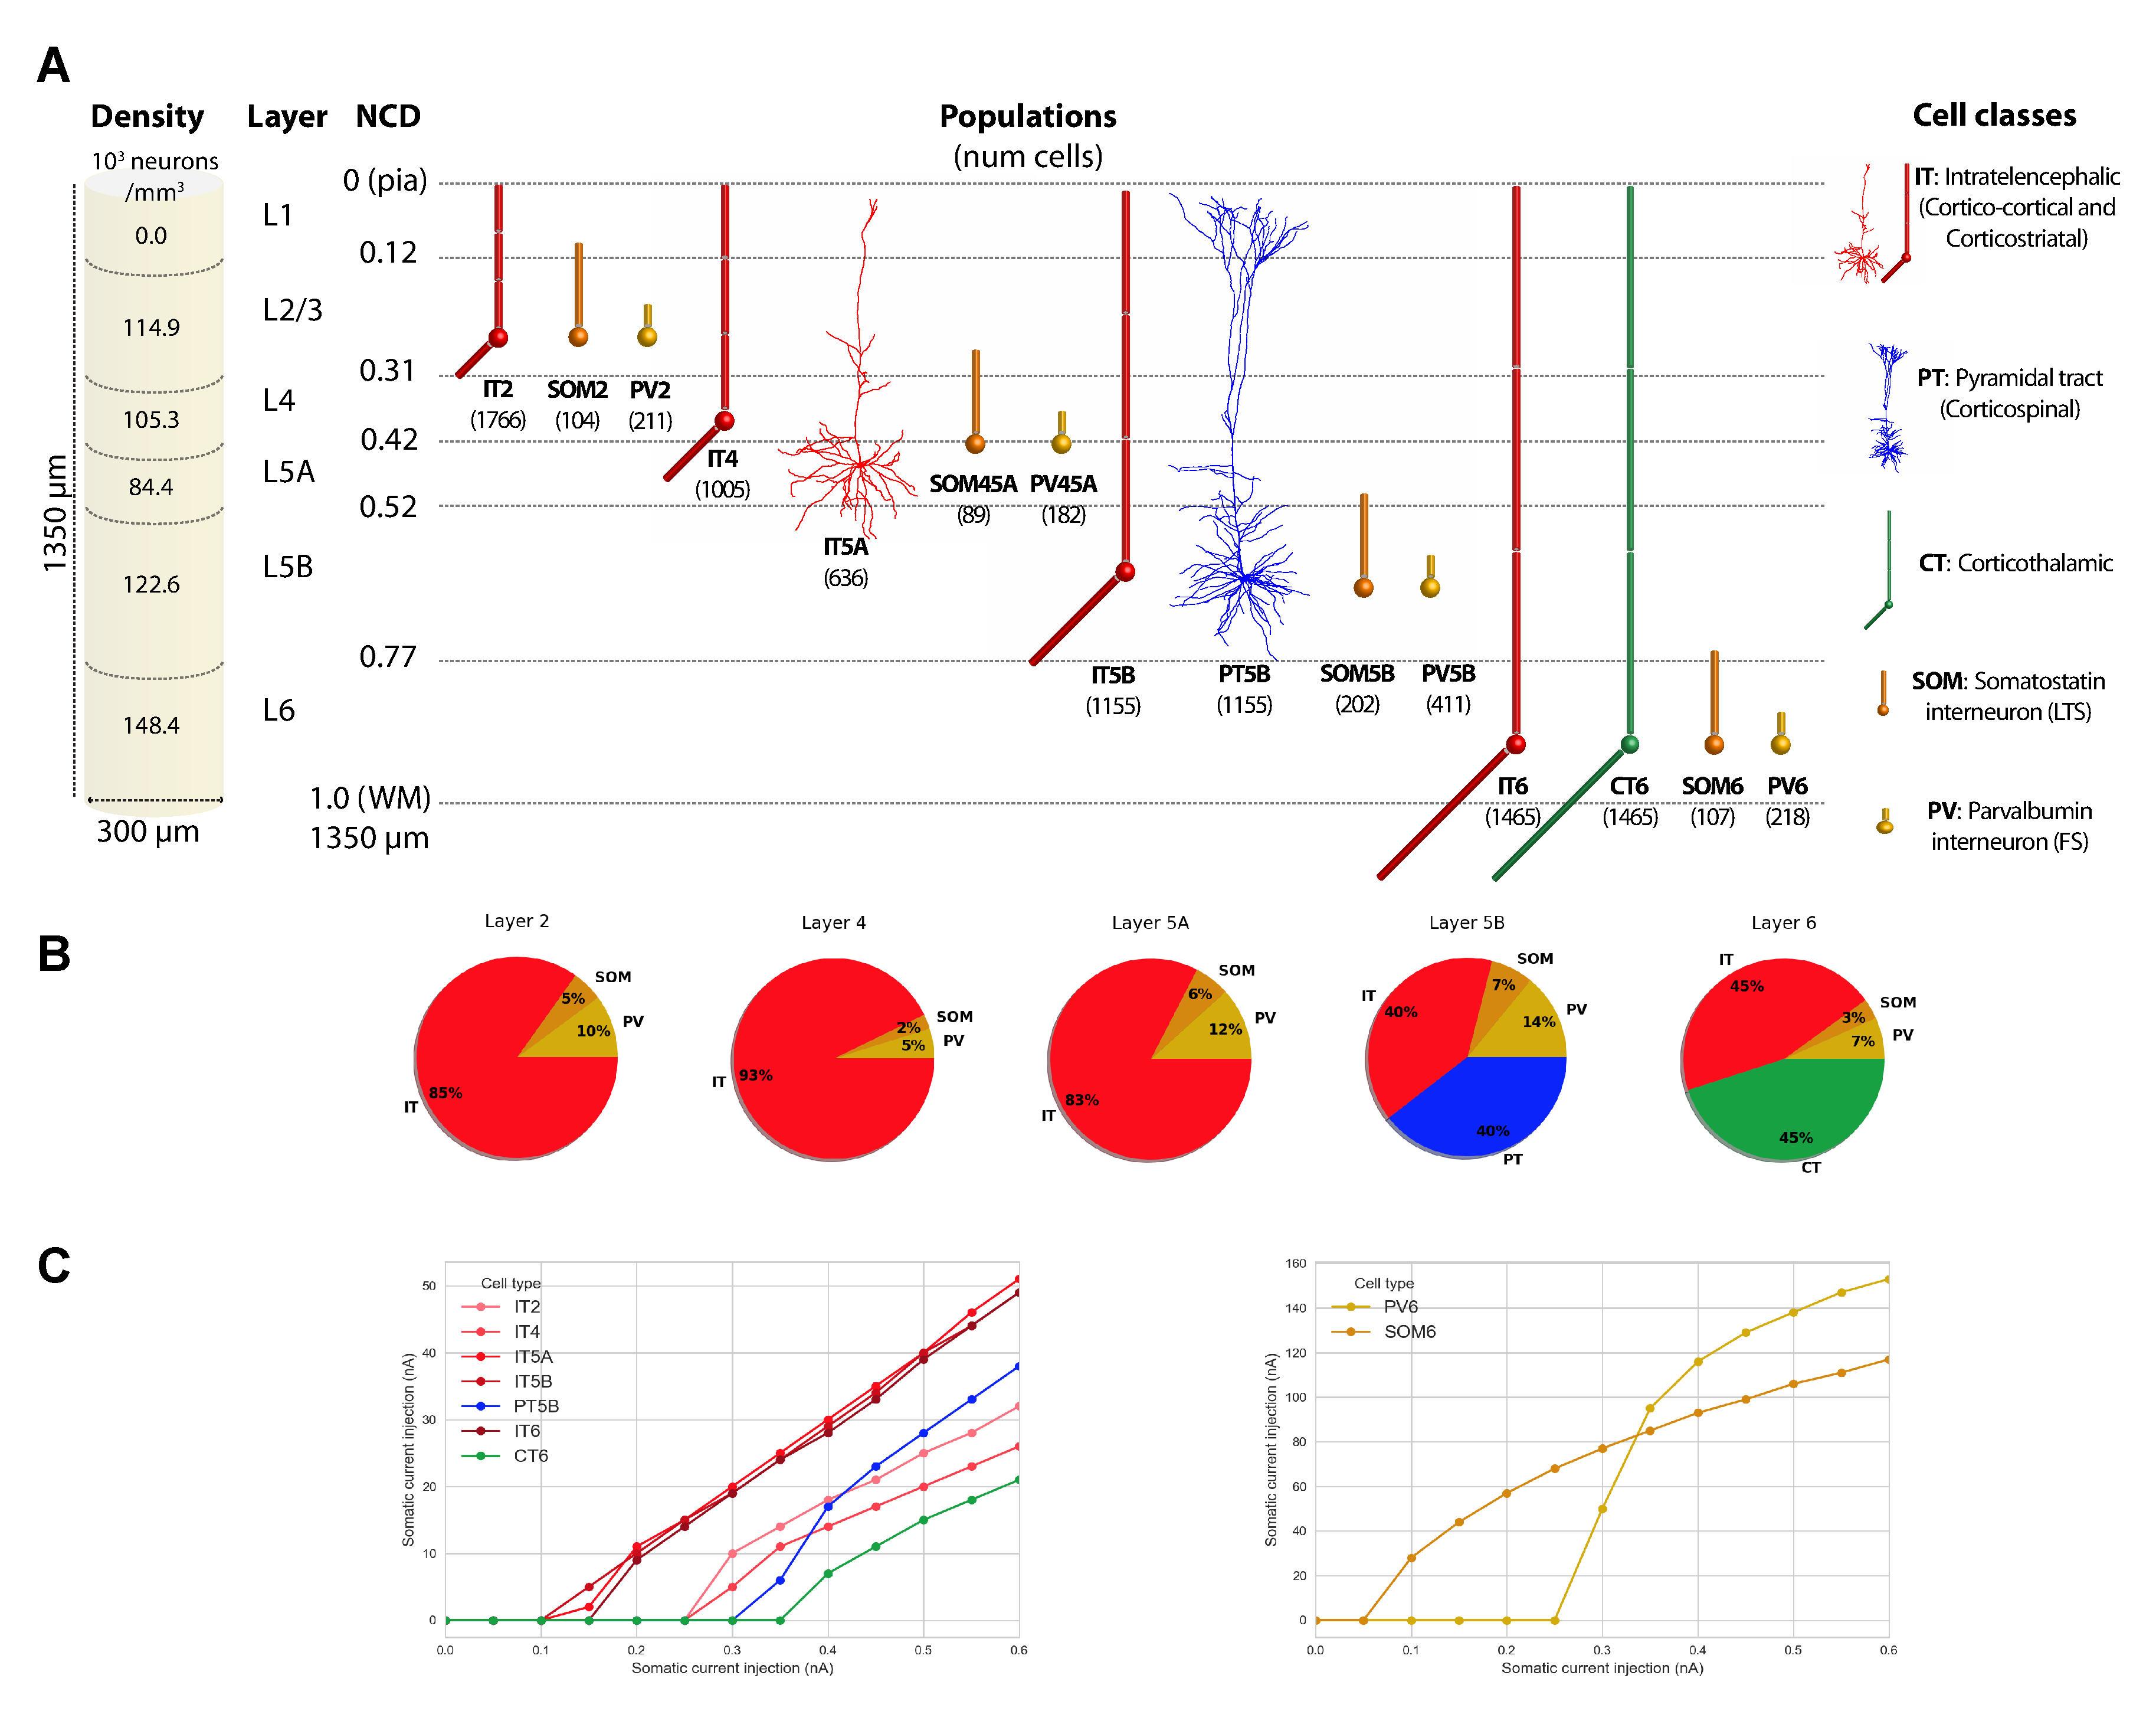
\includegraphics[width=\textwidth]{figs/pops.pdf}
\caption{{\bf Microcircuit dimensions and neuron densities, composition, classes, morphologies and f-I response.}
A) Volume, cell density per layer, populations, number of cells, and morphologies; B) Proportion of cell classes per layer; C) f-I curve for each excitatory and inhibitory cell class.}
\label{fig_pops}
\end{figure}

%%%%%%%%%%%%%%%%%%%%%%%%%%%%%%%%%%%%%%%%%
% Microcircuit composition: neuron locations, densities and ratios
\subsection{Microcircuit composition: neuron locations, densities and ratios}

%% Cylinder dimensions and layers
We modeled in full scale a cylindric volume of mouse M1 cortical microcircuits with a 300 $\mu m$ diameter and 1350 $\mu m$ height (cortical depth) with a total of 10,171 neurons \fref{fig_pops}$A$. The cylinder diameter was chosen to approximately match the horizontal dendritic span of a corticospinal neuron located at the center, consistent with the approach used in the HBP model of rat S1 microcircuits \cite{Mark15}. Mouse cortical depth and boundaries for layers 2/3, 4, 5A, 5B and 6 were based on our published experimental data \cite{Weil08,Ande10,Yama15}. Although traditionally M1 has been considered an agranular area lacking layer 4, we recently identified M1 pyramidal neurons with the expected prototypical physiological, morphological and wiring properties of layer 4 neurons \cite{Yama15}, and therefore incorporated this layer in the model. 

\note{- Markram radius 210um - "The horizontal dimension was defined as the smallest circle required to attain maximal
dendritic volume at a central minicolumn (brown, top); cut- off radius, 95\% of the plateau volume (r = 210 $\mu m$, middle). )
- M1 radius = 150 $\mu m$ (proportional to cortical depth: 1350/2082 * 210 ~=140 $\mu m$)}

%% Neuronal densities, populations and proportions per layer
Cell classes present in each layer were determined based on mouse M1 studies \cite{Harr15,Sute13,Ande10,Yama15,Oswa13,Kons14,Naka16}. IT cell populations were present in all layers, whereas the PT cell population was confined to layer 5B, and the CT cell population only occupied layer 6. SOM and PV interneuron populations were distributed in each layer, with layer 4 and 5B sharing the same populations. Neuronal densities (neurons per $mm^{3}$) for each layer \fref{fig_pops}$A$ were taken from a histological and imaging study of mouse agranaular cortex \cite{Tsai09}. The proportion of excitatory to inhibitory neurons per layer was obtained from mouse S1 data \cite{Lefo09}. The proportion of IT to PT and IT to CT cells in layers 5B and 6, respectively, were both estimated as 1:1 \cite{Harr15,Sute13,Yama15b}. The ratio of PV to SOM neurons per layer was estimated as 2:1 based on mouse M1 and S1 studies \cite{Katz11,WallD16}. The number of cells for each population was calculated based on the modeled cylinder dimensions, layer boundaries and neuronal proportions and densities per layer.

%%%%%%%%%%%%%%%%%%%%%%%%%%%%%%%%%%%%%%%%%
% Local connectivity
\subsection{Local connectivity}

%% Figure: Local connectivity matrices
\begin{figure}[!h]  %% bht
\centering
\includegraphics[width=\textwidth]{figs/conn_local.png}
\caption{{\bf Microcircuit local connectivity. [INCLUDE CIRCUIT DIAGRAM WITH MAIN CONNECTIONS; LABEL LAYERS]}
A) Volume, cell density per layer, populations, number of cells, and morphologies; B) Proportion of cell classes per layer; C) f-I curve for each excitatory and inhibitory cell class.}
\label{fig_conn_local}
\end{figure}

%% E->E, NCD
We calculated local connectivity between M1 neurons \fref{fig_conn_local} by combining data from multiple studies. Data on excitatory inputs to excitatory neurons (IT, PT and CT) was primarily derived from mapping studies using whole-cell recording, glutamate uncaging–based laser-scanning photostimulation (LSPS) and channelrhodopsin-2-assisted circuit mapping (CRACM) analysis \cite{Weil08,Ande10,Yama15,Yama15b}. Connectivity data was postsynaptic cell class-specific and employed normalized cortical depth (NCD) instead of layers as the primary reference system. Unlike layer definitions which are interpreted differently, NCD provides a well-defined, consistent and continuous reference system, depending only on two readily-identifiable landmarks: pia (NCD=0) and white matter (NCD=1). Incorporating NCD-based connectivity into our model allowed us to capture wiring patterns down to a 100 $\mu m$ spatial resolution, well beyond traditional layer-based cortical models. M1 connectivity varied systematically within layers. For example, the strength of inputs from layer 2/3 to L5B corticospinal cells depends significantly on cell soma depth, with upper neurons receiving much stronger input \cite{Ande10}.

%% E->E, postsyn cell specific
Connection strength thus depended on presynaptic NCD and postsynatic NCD and cell class. For postsynaptic IT neurons with NCD ranging from 0.0 to 0.3125 (layer 2/3) and 0.8125 to 1.0 (layer 6) we determined connection strengths based on data from \cite{Weil08} with cortical depth resolution of 140 $\mu m$-resolution. For postsynaptic IT and PT neurons with NCD between 0.3125 and 0.8125 (layers 4, 5A and 5B) we employed connectivity strength data from \cite{Ande10} with cortical depth resolution of 100 $\mu m$. For postsynaptic CT neurons in layer 6 we used the same connection strengths as for layer 6 IT cells \cite{Weil08}, but reduced to 62\% of original values, following published data on the circuitry of M1 CT neurons \cite{Yama15b}. Diagonal elements in the connectivity matrices were increased by 20\% to compensate for the underestimates resulting from LSPS CRACM analysis. Our data \cite{Yama15b} also suggested that connection strength from layer 4 to layer 2/3 IT cells was similar to that measured in S1, so for these projections we employed values from Lefort's S1 connectivity strength matrix \cite{Lefo09}. Experimentally, these connections were found to be four times stronger than in the opposite direction -- from layer 2/3 to layer 4 -- so we decreased the latter in the model to match this ratio.

%% Strength, unitary connection strength (weight), probability; separation
Following previous publications \cite{Kiri12,Lefo09}, we defined connection strength ($s_{con}$) between two populations, as the product of their probability of connection ($p_{con}$) and the unitary connection somatic EPSP amplitude in mV ($i_con$), i.e. $s_{con} = p_{con} \times i_{con}$. We employed this equivalence to disentangle the connection $s_{con}$ values provided by the above LSPS studies into $p_{con}$ and $i_{con}$ values that we could use to implement the model. First, we rescaled the LSPS raw current values in pA \cite{Ande10,Weil08,Yama15,Yama15b} to match $s_{con}$ data from a paired recording study of mouse M1 L5 excitatory circuits \cite{Kiri12}. Next, we calculated the M1 NCD-based $i_{con}$ matrix by interpolating a layerwise unitary connection EPSP amplitude matrix of mouse S1 \cite{Lefo09}, and thresholding values between 0.3 and 1.0 mV. Finally, we calculated the probability of connection matrix as $p_{con} = s_{con} / i_{con}$.  

\note{Detailed steps (Sup info?):
1. For postsynaptic IT neurons in layers 2, 3 use the Weiler rows 1-3 (yfrac centers 0.15, 0.25, 0.35 respectively).

2. 2. For postynaptic IT neurons in layers 4 5A and 5B, use the A&S CSTR matrix (7 rows; 2 rows in L5A, yfrac centers 0.34 and 0.41; 
# 5 rows in L5B, yfrac centers 0.47 to 0.72). For ITs in the deepest part of L5B (yfrac center 0.78), assume input is zero.

3. For postsynaptic PT neurons in layer 5B, use the A&S CSP matrix (6 rows; yfrac centers from 0.47 to 0.78

4. For postsynaptic IT, CT neurons in layer 6, use the Weiler rows 8-9 (yfrac centers 0.85, 0.95 respectively).
# IT->CT / IT->IT6: 0.620 (Yamawaki & Shepherd 2015)

5. Decrease IT5B->IT2, IT5B<->IT5A,IT4 and IT6->IT5B multiplying strength by 0.75, so IT intralaminar > interlaminar

6. Rescale diagonals (increase by 20\%) since underestimated in LSPS data

7a. Increase L4->L2/3 strength based on Yamawaki et al, 2015; suggests similar strength to S1, so use smat L4->L2 from Lefort

7b. Decrease L2/3->L4 strength based on Yamawaki et al, 2015 (~1/4 of L4->L2/3):
- swap high value of bin 0.375-0.4375 (predominantly L2/3->L4) with low value of bin 0.4375-0.5 (predominantly L2/3->L5A)
- decrease strength of L2/3->L4 by 2 so its approx 1/4 of L4->L2/3 (0.117 vs 0.38)

8a. In all cases, truncate negative weights and NaN to 0
8b. Rescale all W+AS data so L5A->L5A equivalent to Kiritani: strength (Icon) = prob(pcon) * unitary weight (icon); scaling factor = 0.04621/2.48 = 0.01863

9. Separation of strength (smat) into probability (pmat) and unitary weight (wmat) 
9.a Rescale Lefort wmat so L5A->L5A approx equivalent to Kiritani
- Use L3, L5A, L5B and L6 weights from Lefort 
- bound Lefort to 0.3 - 1.0 mV (removes outliers due to small sampling size)
9b. Generate wmat based on the rescaled Lefort  - rescale Lefort wmat to W+AS dimensions (using interpolation)
9.c Obtain pmat = smat/wmat
}

%% Weight normalization
To implement $i_{con}$ values in the model we calculated the required NEURON connection weight of an excitatory synaptic input to generate a somatic EPSP of 0.5 mV at each neuron segment. This allowed us to calculate a scaling factor for each segment that converted $i_{con}$ values into NEURON weights, such that the somatic EPSP response to a unitary connection input was independent of synaptic location. This is consistent with experimental evidence showing synpatic conductances increased with distance from soma, to normalize somatic EPSP amplitude of inputs within 300 $\mu m$ of soma \cite{Mage00}. Following this study, scaling factor values above 4.0 -- such as those calculated for PT cell apical tufts -- were thresholded to avoid overexcitability in the network context where each cell receives hundreds of inputs that interact nonlinearly \cite{Spru08,Beha12}. For morphologically detailed cells (layer 5A IT and layer 5B PT), the number of synaptic contacts per unitary connection (or simply, synapses per connection) was set to five, an estimated average consistent with the limited mouse M1 data \cite{HuAg16} and rat S1 studies \cite{Brun06,Mark15}. Individual synaptic weights were calculated by dividing the unitary connection weight ($i_{con}$) by the number of synapses per connection. Although the method does not account for nonlinear summation effects \cite{Spru08}, it provides a reasonable approximation and enables employing a more realistic number and spatial distribution of synapses, which may be key for dendritic computations \cite{Lond05}. For the remaining cell models, all with six compartments or less, a single synapse per connection was used. 

%% E->I and I->E/I
For excitatory inputs to inhibtory cell types (PV and SOM) we started with the same values as for IT cell types but adapted these based on the  specific connectivity patterns reported for mouse M1 interneurons \cite{Apic12,Yama15b} \fref{fig_conn_local}. Following the layer-based description in these studies, we employed three major subdivisions: layer 2/3 (NCD 0.12 to 0.31), layers 4, 5A and 5B (NCD 0.31 to 0.77) and layer 6 (NCD 0.77 to 1.0).  
We increased the probability of layer 2/3 excitatory connections to layers 4, 5A and 5B SOM cells by 50\% and decreased that to PV cells by 50\% \cite{Apic12}. We implemented the opposite pattern for excitatory connections arising from layer 4,5A,5B IT cells such that PV interneurons received stronger intralaminar inputs than SOM cells \cite{Apic12}. The model also accounts for layer 6 CT neurons generating relatively more inhibition than IT neurons \cite{Yama15b}. Inhibitory connections from interneurons (PV and SOM) to other cell types were limited to neurons in the same layer \cite{Katz11}, with layers 4, 5A and 5B combined into a single layer \cite{Naka16}. Probability of connection decayed exponentially with the distance between the pre- and post-synaptic cell bodies with length constant of 100 $\mu m$ \cite{GalL17,Fino11}.

%% Disynaptic inhibition (Yama15)
We biased connectivity towards generating disynaptic inhibition that matched existing excitatory connections in the form $E_1 \rightarrow E_2$ ; $E_1 \rightarrow I \rightarrow E_2$ following data from \cite{Yama15b}. We implemented this by increasing the chance of inhibitory cells targeting excitatory cells that received input from an excitatory cell that also projected to the source inhibitory cell. We set the bias so 90\% of inhibitory connections in layers 4, 5A, 5B, and 6 form disynaptic inhibition. This reduces the level 

% Synapses 
Excitatory synapses consisted of colocalized AMPA (rise, decay $\tau$: 0.05, 5.3 ms) and NMDA (rise, decay $\tau$: 15, 150 ms) receptors, both with reversal potential of 0 mV. The ratio of NMDA to AMPA receptors was 1.0 \cite{Myme03}, meaning their weights were each set to 50\% of the connection weight. NMDA conductance was scaled by $1/(1 + 0.28 · Mg · \exp{(−0.062 · V))}$; Mg = 1mM \cite{jahr1990voltage}. Inhibitory synapses from SOM to excitatory neurons consisted of a slow GABAA receptor (rise, decay $\tau$: 2, 100 ms) and GABAB receptor, in a 90\% to 10\% proportion; synapses from SOM to inhibitory neurons only included the slow GABAA receptor; and synapses from PV to other neurons consisted of a fast GABAA receptor (rise, decay $\tau$: 0.07, 18.2). The reversal potential was -80 mV for GABAA and -95 mV for GABAB. The GABAB synapse was modeled using second messenger connectivity to a G protein-coupled inwardly-rectifying potassium channel (GIRK) \cite{destexhe96a}. The remaining synapses were modeled with a double-exponential mechanism. 

% Delays
Connection delays were estimated as 2 ms plus a variable delay depending on the distance between the pre- and postsynaptic cell bodies assuming a propagation speed of 0.5 m/s.


%%%%%%%%%%%%%%%%%%%%%%%%%%%%%%%%%%%%%%%%%
% Long-range input connectivity
\subsection{Long-range input connectivity}

%% Figure: Long range inputs
\begin{figure}[!h]  %% bht
\centering
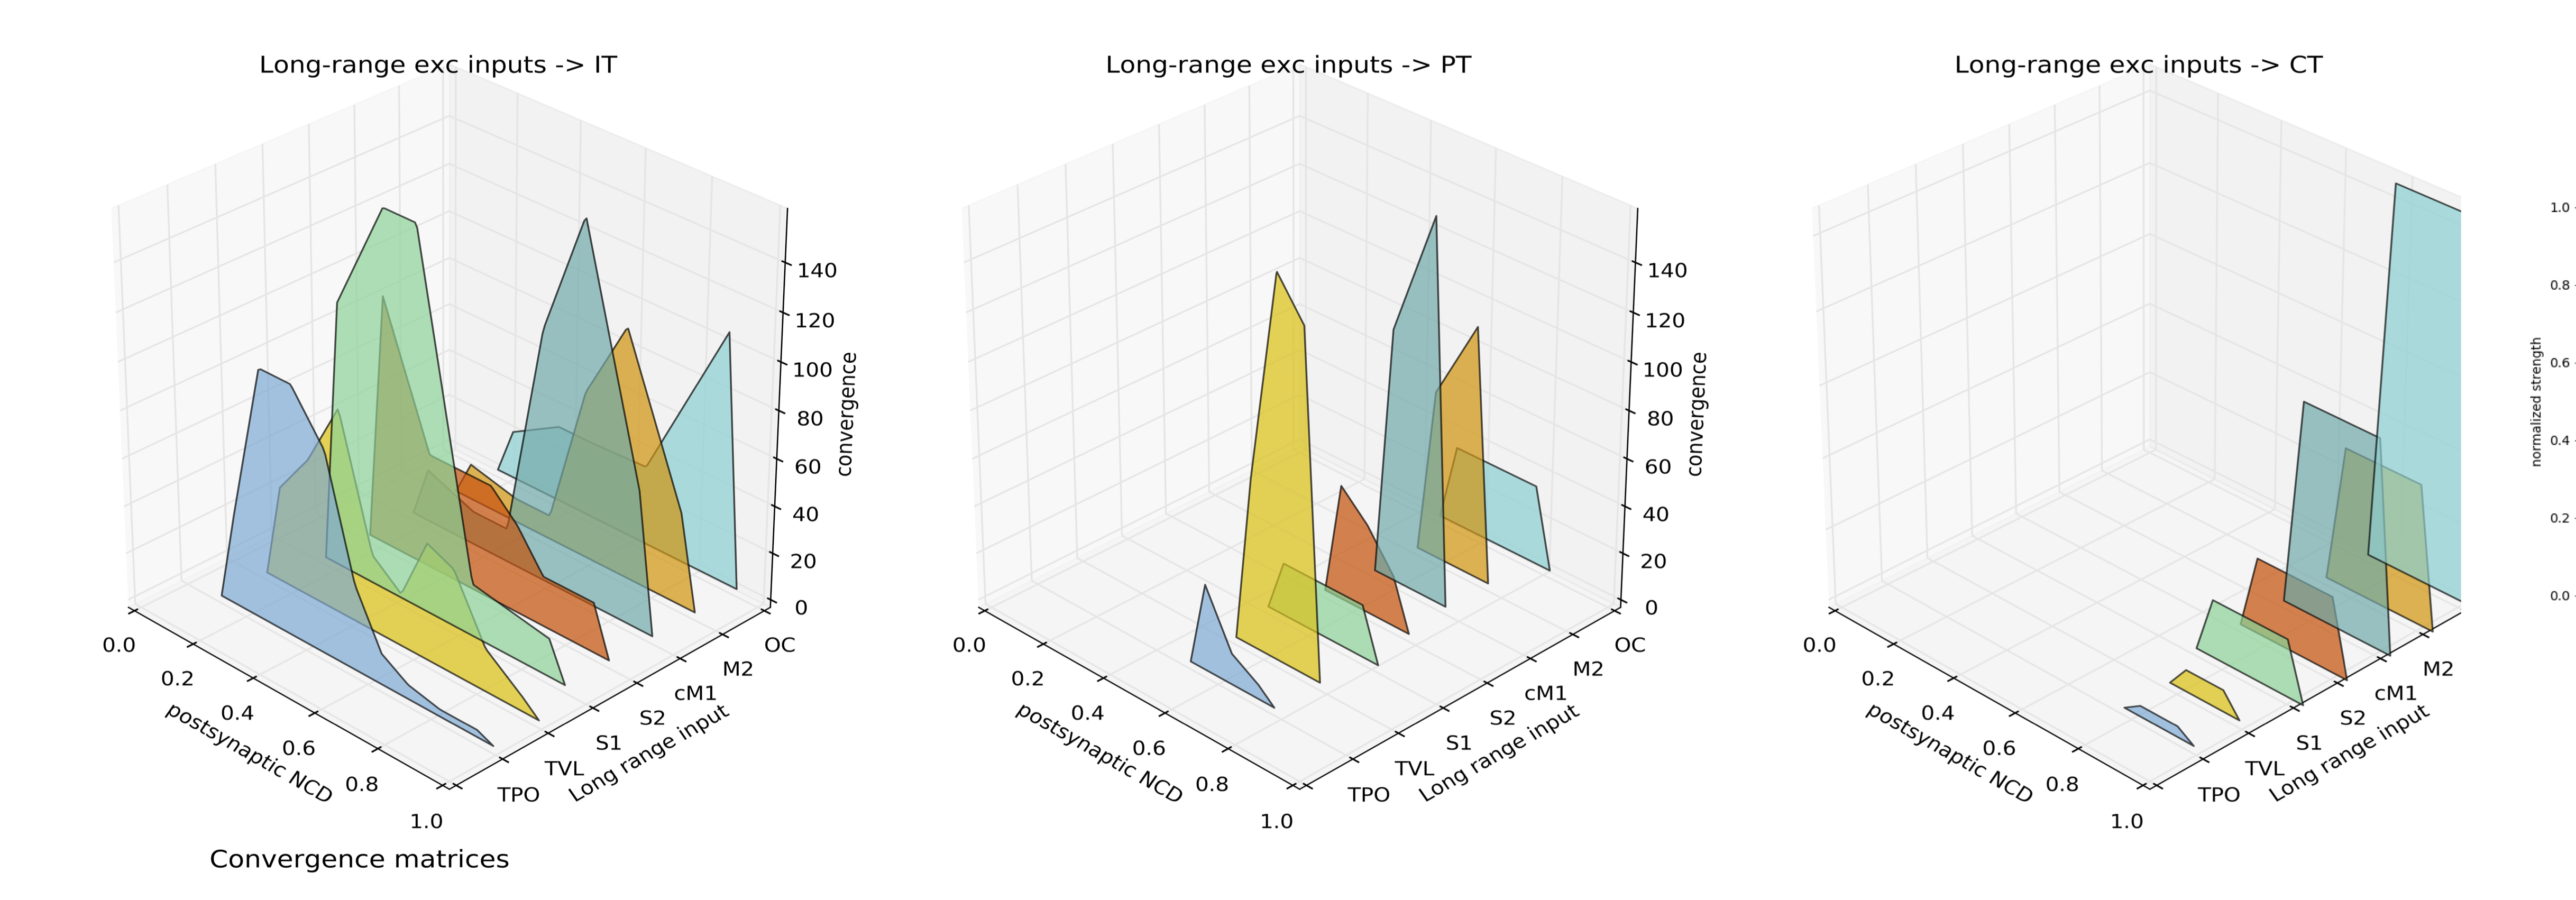
\includegraphics[width=\textwidth]{figs/conn_long.png}
\caption{{\bf Long-range inputs to M1 microcircuit.}
}
\label{fig_conn_long}
\end{figure}

%% Conn pattern from each region
We added long-range input connections from seven regions that are known to project to M1: thalamus posterior nucleus (TPO), ventro-lateral thalamus (TVL), primary somatosensory cortex (S1), secondary somatosensory cortex (S2), contralateral primary motor cortex (cM1), secondary motor cortex (M2) and orbital cortex (OC). Each region consisted of a population of 1000 \cite{Cons13,Brun06} spike-generators (NEURON VecStims) that generated independent random Poisson spike trains with uniform distributed rates between 0 and 2 Hz \cite{Yama13,Hira06}; or 0 to 20 Hz \cite{Isom09,Jaco12} when simulating increased input from a region. Previous studies -- using the LSPS CRACM method -- provided a measure of  normalized input strength from these regions as a function of postsynaptic cell type and layer or NCD. Broadly, TPO \cite{Yama15,Yama15b,Naka16}, S1 \cite{MaoK11} and S2 \cite{Sute15} projected strongly to IT cells in layers 2/3, 4 and 5A; TVL projected strongly to PT cells and moderately to IT cells \cite{Yama15,Yama15b,Naka16}; cM1 and M2 projected strongly to IT and PT cells in layers 5B and 6 \cite{Hook13}; and OC projected strongly to layer 6 CT and IT cells \cite{Hook13}. We implemented these relations by estimating the maximum number of synaptic inputs from each region and multiplying that value by the normalized input strength for each postsynaptic cell type and NCD range. This resulted in a convergence value -- average number of synaptic inputs to each postsynaptic cell -- for each projection \fref{fig_conn_long}. We fixed all connection weights (unitary connection somatic EPSP amplitude) to 0.5 mV, consistent with rat and mouse S1 data \cite{HuAg16,Cons13}.

%% assumptions to calculate convergence
To estimate the maximum number of synaptic inputs per region, we made a number of assumptions based on the limited data available \fref{fig_conn_long}. First, we estimated the average number of synaptic contacts per cell as 8234 by rescaling rat S1 data \cite{Meye10} based on our own observations for PT cells \cite{Sute13} and contrasting with related studies \cite{Schu89,DeFe02}; we assumed the same value for all cell types so we could use convergence to approximate long-range input strength. We assumed 80 \% of synaptic inputs were excitatory vs. 20 \% inhibitory \cite{DeFe02,Mark15}; out of the excitatory inputs, 80 \% were long-range vs. 20 \% local \cite{Mark15,Step09}; and out of the inhibitory inputs, 30 \% were long-range vs. 70 \% local \cite{Step09}. Finally, we estimated the percentage of long-range synaptic inputs arriving from each region based on mouse brain mesoscale connectivity data \cite{OhHa14} and other studies \cite{Meye10b,Brun06,Meye10,Zhan16,Bopp17}: TVL, S1, cM1 each contributed 15 \%, whereas TPO, S2, M2 and OC each accounted for 10 \%. 


%%%%%%%%%%%%%%%%%%%%%%%%%%%%%%%%%%%%%%%%%
% Dendritic distribution of synaptic inputs
\subsection{Dendritic distribution of synaptic inputs}

%% Figure: Dendritic distribution
\begin{figure}[!h]  %% bht
\centering
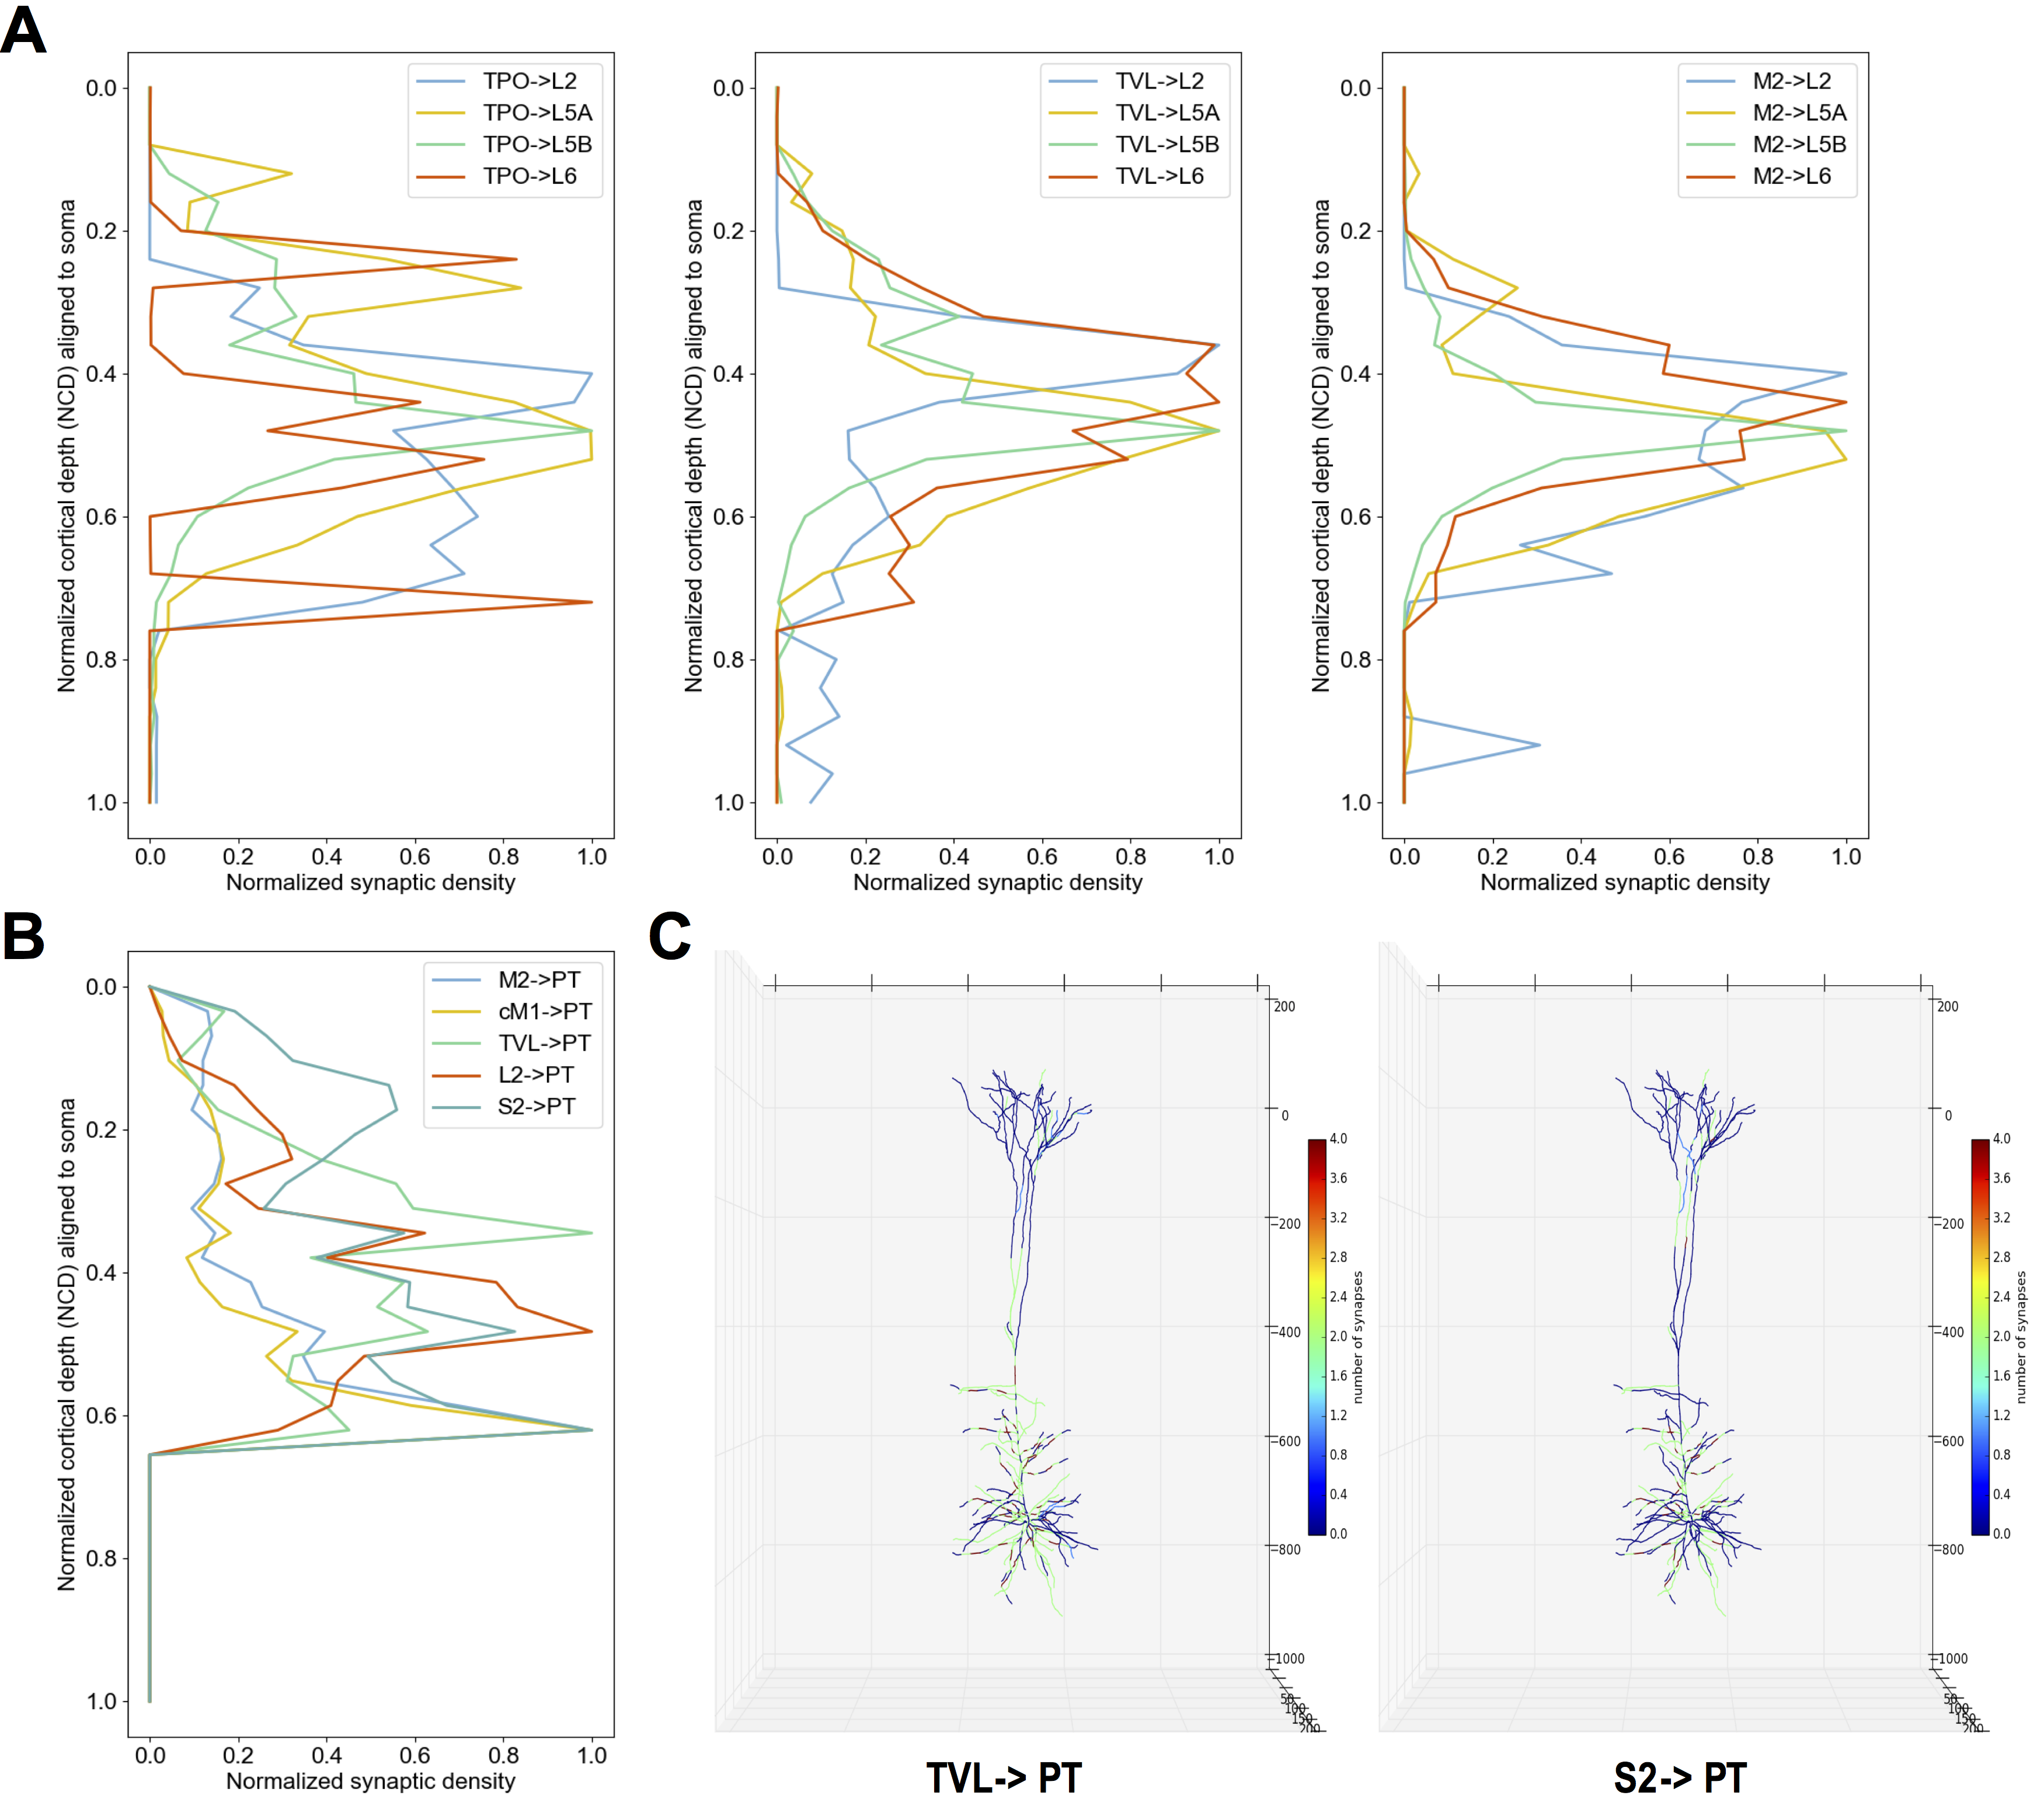
\includegraphics[width=\textwidth]{figs/conn_dend.png}
\caption{{\bf Dendritic distribution of synaptic inputs.}
}
\label{fig_conn_dend}
\end{figure}

Experimental evidence demonstrates the location of synapses along dendritic trees follows very specific patterns of organization that depend on the brain region, cell type and cortical depth \cite{Petr09,Sute15}; these are likely to result in important functional effects \cite{Kubo15,Laud14,Spru08}. We employed subcellular Channelrhodopsin-2-Assisted Circuit Mapping (sCRACM) data to estimate the synaptic density along the dendritic arbor -- 1D radial axis -- for inputs from TPO, TVL, M2 and OC to layers 2/3, 5A, 5B and 6 IT and CT cell \cite{Hook13} (\fref{fig_conn_dend}A), and from layer 2/3 IT, TVL, S1, S2, cM1 and M2 to PT neurons \cite{Sute15} (\fref{fig_conn_dend}B). To approximate radial synaptic density we divided the sCRACM map amplitudes by the dendritic length at each grid location, and averaged across rows. Once all network connections had been generated, synaptic locations were automatically calculated for each cell based on its morphology and the pre- and postsynaptic cell type-specific radial synaptic density function (\fref{fig_conn_dend}C). Synaptic inputs from PV to excitatory cells were located perisomatically (50 $\mu m$ around soma); SOM inputs targeted apical dendrites of excitatory neurons \cite{Naka16,Katz11}; and all inputs to PV and SOM cells targeted apical dendrites. For projections where no data synaptic distribution data was available -- IT/CT, S1, S2 and cM1 to IT/CT cells -- we assumed a uniform dendritic length distribution. 

%%%%%%%%%%%%%%%%%%%%%%%%%%%%%%%%%%%%%%%%%
% Model implementation, simulation and analysis
\subsection{Model implementation, simulation and analysis}

%% NEURON and NetPyNE
The model was developed using parallel NEURON \cite{Lytt16b} and NetPyNE \cite{Dura16c} (www.neurosimlab.org/netpyne), a Python package to facilitate the development of biological neuronal networks in the NEURON simulator. NetPyNE emphasizes  the incorporation of multiscale anatomical and physiological data at varying levels of detail. It converts a set of simple, standardized high-level specifications in a declarative format into a NEURON model. NetPyNE also facilitates organizing and running parallel simulations by taking care of distributing the workload and gathering data across computing nodes. It also provides a powerful set of analysis methods so the user can plot spike raster plots, LFP power spectra, information transfer measures, connectivity matrices, or intrinsic time-varying variables (eg. voltage) of any subset of cells. To facilitate data sharing, the package saves and loads the specifications, network, and simulation results using common file formats (Pickle, Matlab, JSON or HDF5), and can convert to and from NeuroML, a standard data format for exchanging models in computational neuroscience. Simulations were run on XSEDE supercomputers Comet and Stampede using the Neuroscience Gateway (NSG) and our own resource allocation. 
\note{batch simulations, explorations; num cores per sim; num sims per batch; total cores; total hours used; efficient simulation}


%%% Local Variables: 
%%% mode: latex
%%% TeX-master: "main.tex"
%%% End:


